appendix/rcuimplCUinLinux.tex

\chapter{Read-Copy Update in Linux}
\label{app:rcuhist:Read-Copy Update in Linux}

\OriginallyPublished{Appendix}{app:rcuhist:Read-Copy Update in Linux}{Read-Copy Update in Linux}{ACM Operating Systems Review}{PaulEMcKenney2008RCUOSR}

Authors: Paul E. McKenney and Jonathan Walpole

There can be no doubt that a great many technologies have been
added to Linux over the past ten years.
What is less well-known is that it is often necessary to
introduce a large amount of Linux into a given technology in order
to successfully introduce that technology into Linux.
This chapter illustrates such an introduction of Linux into
technology with Read-Copy Update (RCU).
The RCU API's evolution over time clearly shows that Linux's
extremely diverse set of workloads and platforms has
changed RCU to a far greater degree than RCU has changed
Linux---and it
is reasonable to expect that other technologies that might
be proposed for inclusion into Linux would face similar challenges.
In addition, this paper presents a summary of lessons learned and
an attempt to foresee what additional challenges Linux
might present to RCU.

\section{Introduction to RCU in Linux}
\label{sec:app:rcuhist:Introduction to RCU in Linux}

Linux is an operating-system kernel that is used in a variety of
platforms ranging from cellphones to super-computers,
with more than an 80\% share of the Top 500 Supercomputer Sites
as of November 2007~\cite{Top500byOS}, up from about 10\% in late 2000.
Although a very large amount of functionality has been added to the
Linux kernel between 2000 and 2007, space constraints limit this paper to
discussing but one specific niche technology, namely RCU.
We shall see that the extreme diversity of Linux's platforms and
workloads posed special challenges to RCU.
It seems likely that this diversity would pose similar challenges to
other technologies that might be proposed for inclusion into the
Linux kernel.

Section~\ref{sec:app:rcuhist:RCU Usage Within Linux}
gives a quantitative summary of RCU's use by the Linux kernel since
its acceptance in late 2002,
and Section~\ref{sec:app:rcuhist:RCU Before Linux} gives an overview of RCU and
its environment in production systems prior to its acceptance into Linux.
Section~\ref{sec:app:rcuhist:Evolution of the RCU API}
reviews the evolution of the RCU API in the Linux kernel, and
Section~\ref{sec:app:rcuhist:Lessons Learned}
delineates some of the forces underlying this evolution.
Section~\ref{sec:app:rcuhist:Future Prospects}
presents some speculation on the future evolution of the RCU API,
and
Section~\ref{sec:app:rcuhist:Conclusions}
presents concluding remarks.
Finally, Section~\ref{sec:app:rcuhist:Epilog} contains RCU history subsequent to
this paper's initial publication in
SIGOPS Operating Systems Review~\cite{PaulEMcKenney2008RCUOSR}.

\section{RCU Usage Within Linux}
\label{sec:app:rcuhist:RCU Usage Within Linux}

\begin{figure}[tb]
\begin{center}
\resizebox{3in}{!}{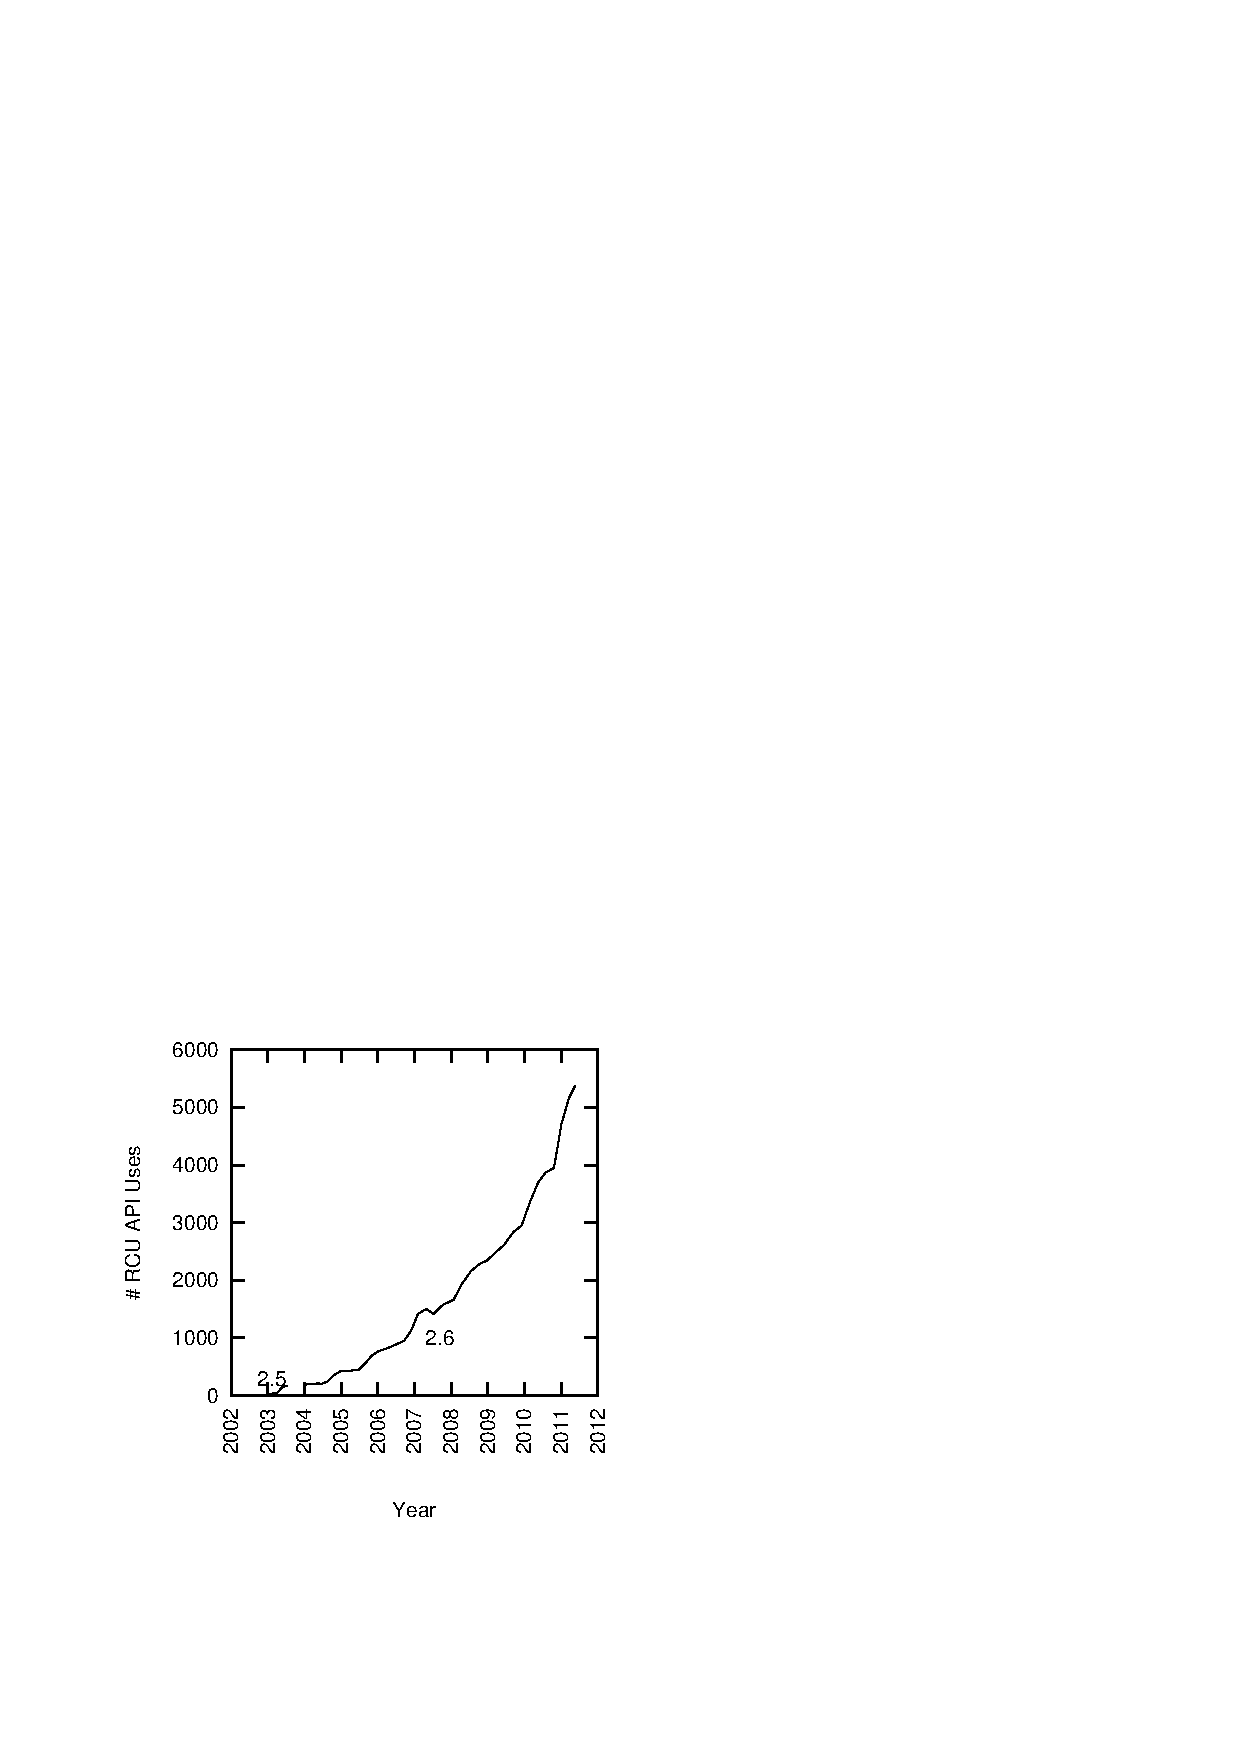
\includegraphics{appendix/rcuhist/linux-RCU}}
\end{center}
\caption{RCU API Usage in the Linux Kernel}
\label{fig:app:rcuhist:RCU API Usage in the Linux Kernel}
\end{figure}

\begin{figure}[tb]
\begin{center}
\resizebox{3in}{!}{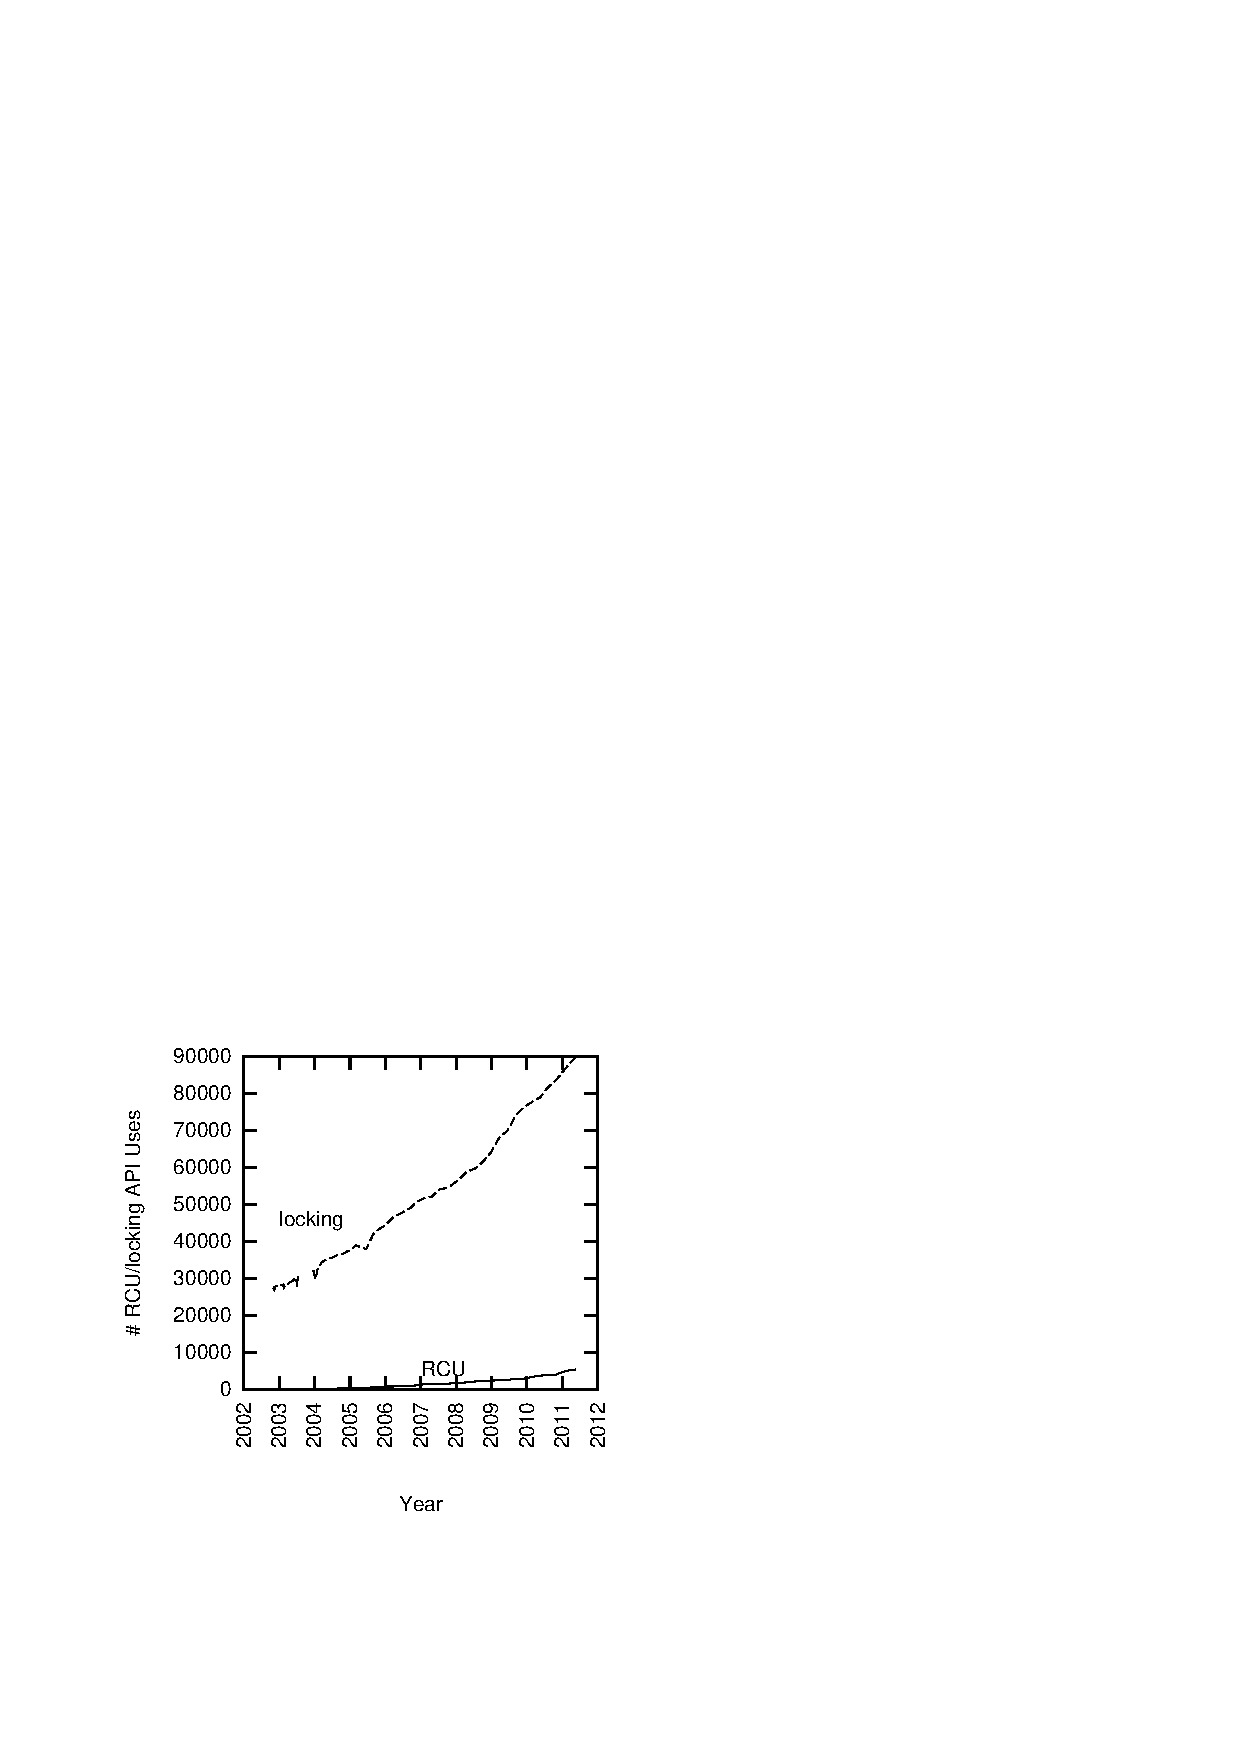
\includegraphics{appendix/rcuhist/linux-RCUlock}}
\end{center}
\caption{RCU API Usage in the Linux Kernel vs. Locking}
\label{fig:app:rcuhist:RCU API Usage in the Linux Kernel vs. Locking}
\end{figure}

RCU's usage within the Linux kernel has increased rapidly over the past
five years, as shown in
Figure~\ref{fig:app:rcuhist:RCU API Usage in the Linux Kernel}~\cite{PaulEMcKenneyRCUusagePage}.
In some cases, RCU has displaced other synchronization mechanisms
in existing code
(for example, \co{brlock} in the networking protocol
stacks~\cite{Molnar00a,Torvalds2.5.69,Torvalds2.5.70}),
while in other cases it has been introduced with code implementing
new functionality
(for example, the audit system within SELinux~\cite{JamesMorris04b}).
Despite its rapid growth, RCU remains a niche technology,
as shown by the comparison with locking in
Figure~\ref{fig:app:rcuhist:RCU API Usage in the Linux Kernel vs. Locking}.
Nonetheless, RCU can be characterized as a reasonably successful
niche technology within the Linux kernel.
As such, it is useful to review the path RCU took in achieving this
modest level of success, which was due more to RCU's being
dramatically changed by Linux than by Linux being changed by RCU.

\section{RCU Before Linux}
\label{sec:app:rcuhist:RCU Before Linux}

Before Linux, production use of RCU-like mechanisms appears to have been
confined to large data-processing systems such as the
IBM mainframe's VM/XA~\cite{Hennessy89} and Sequent's (now IBM's)
Symmetry and NUMA-Q systems running the DYNIX/ptx operating
system~\cite{McKenney98}.
These were large (for the time) enterprise systems running parallel
data-processing workloads.
These systems normally ran in a protected networking environment,
behind firewalls or client machines with restricted usage modes.
The real-time response required of these machines is perhaps best
exemplified by the TPC/A benchmark~\cite{TPCA1989}, which has the
very soft real-time requirement
that 90\% of transactions complete in two seconds or less.

Back when the author (Paul) was still foolish enough to believe that
he knew all
that there was to know about RCU,
the RCU API for DYNIX/ptx~\cite{McKenney01b} consisted of only
the following members (translated to their Linux equivalents,
where available):
\begin{enumerate}
\item	\co{rcu_read_lock()}, which marks the beginning of an
	RCU read-side critical section,
\item	\co{rcu_read_unlock()}, which marks the end of an RCU
	read-side critical section,
\item	\co{call_rcu()}, which invokes a specified function after
	all pre-existing RCU read-side critical sections
	have completed,
\item	\co{kfree()}, which frees an unadorned block of memory,
\item	\co{kmem_cache_free()}, which frees a typed block of memory, and
\item	\co{kmem_deferred_free()}, which frees an untyped block of
	memory some time after all pre-existing RCU read-side
	critical sections have completed.
	(This primitive is not available in Linux, as it turns out
	to be simpler to open-code it.)
\end{enumerate}
In addition, this variant of the RCU API made use of explict
memory barriers~\cite{PaulMcKenney2005i}.

The next section describes how the Linux kernel's RCU API evolved over time.

\section{Evolution of the RCU API}
\label{sec:app:rcuhist:Evolution of the RCU API}

\begin{table}[tb]
\begin{center}
\begin{tabular}{l|l}
	Section & Cause of Change \\
	\hline
	\hline
	\ref{sec:app:rcuhist:Simplicity} & Simplicity \\
	\hline
	\ref{sec:app:rcuhist:Memory Barriers Unloved, Part I} &
		Memory Barriers Unloved, Part I \\
	\hline
	\ref{sec:app:rcuhist:Real-Time Systems, Part I} &
		Real-Time Systems, Part I \\
	\hline
	\ref{sec:app:rcuhist:Small-Memory Systems} &
		Small-Memory Systems \\
	\hline
	\ref{sec:app:rcuhist:Heavy Networking Loads} &
		Heavy Networking Loads \\
	\hline
	\ref{sec:app:rcuhist:Network-Based Denial-of-Service Attacks} &
		Network-Based Denial-of-Service Attacks \\
	\hline
	\ref{sec:app:rcuhist:Memory Barriers Unloved, Part II} &
		Memory Barriers Unloved, Part II \\
	\hline
	\ref{sec:app:rcuhist:Linux Accepts RCU's Namesake} &
		Linux Accepts RCU's Namesake \\
	\hline
	\ref{sec:app:rcuhist:Real-Time Systems, Part II} &
		Real-Time Systems, Part II \\
	\hline
	\ref{sec:app:rcuhist:Unloadable Kernel Modules Use RCU} &
		Unloadable Kernel Modules Use RCU \\
	\hline
	\ref{sec:app:rcuhist:RCU Readers Must Block} &
		RCU Readers Must Block \\
	\hline
	\ref{sec:app:rcuhist:RCU Readers of Lists Being Reaped} &
		RCU Readers of Lists Being Reaped \\
	\hline
	\ref{sec:app:rcuhist:Summary of RCU API Evolution} &
		Summary of RCU API Evolution \\
\end{tabular}
\end{center}
\caption{Evolution of the Linux-Kernel RCU API}
\label{tab:app:rcuhist:Evolution of the Linux-Kernel RCU API}
\end{table}

The RCU API has not evolved continuously, but rather in a manner
reminiscent of punctuated equilibrium.
Each burst of API change has had its own distinct motivation,
including simplicity, distaste for explicit memory barriers,
real-time response, memory conservation, networking loads,
kernel modules that can be unloaded, and several specific algorithmic needs.
Each such burst is covered in chronological order in the following sections,
as summarized in
Table~\ref{tab:app:rcuhist:Evolution of the Linux-Kernel RCU API}.

\subsection{Simplicity}
\label{sec:app:rcuhist:Simplicity}

The first force to act on the RCU API was the Linux community's unusually
vociferous preference for simplicity.
Of course, almost everyone prefers simplicity, but will normally accept
a complex solution if it is the only solution known.
In contrast, the Linux community often insists
that a simpler solution be invented.
Such a solution is in fact invented surprisingly frequently.
Any technology being proposed for inclusion into Linux can therefore
expect to face this challenge.

This demand for simplicity first manifested itself
as a demand for an minimal API.
Because the early RCU implementations used context switches to determine
when pre-existing RCU read-side critical sections had completed, and
because early Linux kernels were non-preemptible, the read-side
primitives ~\co{rcu_read_lock()}~
and ~\co{rcu_read_unlock()}
generated no code.
This fact
accounts for their extreme performance and scalabilty: free is indeed
a very good price.
However, it also caused the Linux community to
insist that these primitives be eliminated (temporarily, as it turns out).

The \co{kmem_deferred_free()} primitive provided a safe way
of freeing RCU-protected data elements in face of concurrent RCU readers.
However, because
open-coding this primitive turned out very nearly as simple as invoking
\co{kmem_deferred_free()},
this primitive was also eliminated.
In essence, an API designed to simplify the developer's life turned out
to provide almost no simplification!

On the other hand, this drive for simplicity provided
the easier-to-use
\co{synchronize_kernel()} as an alternative to the
asynchronous \co{call_rcu()}.
The \co{synchronize_kernel()} primitive blocks until all pre-existing
RCU read-side critical sections complete.
However, \co{synchronize_kernel()} could not completely replace
\co{call_rcu()} because as blocking is not permitted within
interrupt handlers.

Although this vociferous demand for simplicity can be painful at times, it can
also be quite beneficial, and might in fact account for much of Linux's
popularity.
After all, if you know only one way to implement something, it is likely
to be neither the simplest nor the most optimal approach.
The spirited discussions conducted in the Linux community often
uncover solutions that are much simpler, faster, and more capable
than those originally proposed.
And in fact a number of RCU implementations were created during this time,
including those from Andi Kleen, Rusty Russell, and Andrea Arcangeli,
with Dipankar Sarma doing the heavy lifting required to compare
them and combine their best features into the implementation that
was eventually accepted into the
Linux kernel~\cite{Arcangeli03,McKenney01a,McKenney02a,Torvalds2.5.43}.

\subsection{Memory Barriers Unloved, Part I}
\label{sec:app:rcuhist:Memory Barriers Unloved, Part I}

Given an operating system with a small developer community and that
runs on but a single CPU family, a good strategy might be to ensure that all
the developers understand how to correctly use facilities such as
memory barriers~\cite{Gharachorloo95}.
Memory barriers enforce ordering of memory references on weakly ordered
multiprocessor systems and on systems with aggressive optimizing
compilers, both of which can change the order in which code is executed.
The correct use of memory barriers is somewhat of
a black art, but an art that is critical to the creation of high-performance
shared-memory-parallel operating-system kernels.
Although only performance-critical technologies are
likely to face this memory-barrier challenge, operating-system kernels
tend to have more than their share of situations where performance
is critical.

However, the above global-understanding strategy
fails to scale,
both with the number of maintainers and with the number of CPU architectures.
In fact, in the case of memory barriers, a number of Linux-kernel
maintainers have at times enforced a blanket policy rejecting any patch
adding an explicit memory barrier to the Linux kernel.
More recently, the \co{checkpatch.pl} patch-vetting script (found in
the \co{scripts} directory in the Linux-kernel source tree)
rejects any patch that adds a memory barrier lacking
an explanatory comment.

In the case of Linux, with thousands of developers and more than 20
CPU families, an even better strategy is to do away with the need
for explicit memory barriers, preferably by burying them into an
easy-to-use higher-level API.
To this end, Manfred Spraul recommended adding new RCU-protected
linked-list primitives that contained any needed
memory barriers~\cite{Spraul01},
relieving Linux kernel developers of the need to consider RCU-related
memory barriers, at least when using Linux's circular doubly linked lists.
The primitives \co{list_for_each_entry_rcu()} (which iterates through
the specified list),
\co{list_add_rcu()} (which adds an item to the beginning of the specified
list),
\co{list_add_tail_rcu()} (which adds to the end),
and \co{list_del_rcu()} (which deletes the specified item)
were duly added to the RCU API.

These additions eliminated the need for explicit memory barriers in code
using RCU-protected lists, freeing the kernel developers from the need
to concern themselves with the memory model provided by
the underlying hardware.
This represented a great leap forward in readability of code using
RCU-protected lists.
Code using other types of RCU-protected data structures was dealt with
later, as described in Section~\ref{sec:app:rcuhist:Memory Barriers Unloved, Part II}.

\subsection{Real-Time Systems, Part I}
\label{sec:app:rcuhist:Real-Time Systems, Part I}

Specially modified versions of Linux have been used for real-time computing
since the mid-to-late 1990s.
Of course, each such version of Linux was subtly different, and
considerable development effort was expended creating
very similar functionality.
This situation called out for the addition of real-time functionality
to the mainline Linux kernel.

An important step towards this goal occurred early in the 2.5 development
effort with the introduction of the \co{CONFIG_PREEMPT} configuration
option, which improved the Linux kernel's real-time response by
introducing kernel preemption.
Unfortunately, all of the Linux RCU implementations at that time assumed a
non-preemptible kernel, as they relied on context switches to determine
when all pre-existing RCU readers had completed.
A simple fix was to cause RCU readers to disable preemption across
RCU read-side critical sections, reintroducing the (nestable)
\co{rcu_read_lock()} and \co{rcu_read_unlock()} primitives.
The outermost \co{rcu_read_lock()} and \co{rcu_read_unlock()}
disable and enable preemption, respectively.

This change enabled RCU to be used in
real-time environments that required millisecond-scale scheduling latencies.
It is reasonable to expect that many concurrency technologies will face
real-time response challenges, particularly those based on
backoff or retry techniques.

\subsection{Small-Memory Systems}
\label{sec:app:rcuhist:Small-Memory Systems}

Linux is used on numerous embedded platforms, which often have
tight constraints on system memory, particularly for platforms
that are powered by batteries.
These small-memory platforms will likely pose special challenges for any
technology constructed using infinite-memory assumptions.
On such platforms, Linux's circular doubly linked lists consume
two pointers worth of memory per hash bucket, which can be problematic
for large hash tables.
Such large hash tables can also be problematic on large-memory systems
with small CPU caches.

Andi Kleen therefore implemented \co{hlist}, which is a linear
doubly linked list.
Although each element still requires two pointers, one in each direction,
each bucket of a hash table need only have a single pointer to the first
element of the list, as opposed to the pair of pointers required for a
list header for a circular doubly linked list.
This reduction from two pointers per hash bucket down to a single pointer
per hash bucket halves the memory consumed by the bucket array making
up a large hash table, which can be the dominating factor in lightly
loaded hash tables optimized for fast lookup.
However, it also required Andi
to also introduce the to the RCU API the primitives
\co{hlist_for_each_entry_rcu()} (which iterates through the specified
\co{hlist}),
\co{hlist_del_rcu()} (which deletes the specified \co{hlist} element),
\co{hlist_add_after_rcu()} (which adds a new entry after the specified
\co{hlist} element),
\co{hlist_add_before_rcu()} (which adds a new entry before the specified
\co{hlist} element), and
\co{hlist_add_head_rcu()} (which adds a new entry to the head of the
specified \co{hlist}).

The addition of these APIs greatly improved performance of some
filesystem workloads on systems with small CPU caches.

\subsection{Heavy Networking Loads}
\label{sec:app:rcuhist:Heavy Networking Loads}

The Linux 2.4 networking
stack used a \co{brlock} primitive based on per-CPU reader-writer locks
(similar to Hsieh's and Weihl's scalable reader-writer
locks~\cite{WilsonCHsieh92a}).
Updaters write-acquired and then immediately write-released this lock,
guaranteeing that all pre-existing readers had completed, a use that
is similar to RCU.
Steve Hemminger therefore replaced this \co{brlock} primitive with RCU,
introducing \co{synchronize_net()} to ease the transition (and
also to ease a transition back, if need be).
This primitive was retained after the transition proved successful,
which permitted \co{brlock} to be eliminated.
However, \co{synchronize_net()} remains a useful documentation aid,
despite its being simply a synonym for \co{synchronize_kernel()}:
both primitives wait for all pre-existing RCU read-side critical
sections to complete.

This change reduced the number of distinct synchronization primitives
in the Linux kernel by eliminating \co{brlock}.

\subsection{Network-Based Denial-of-Service Attacks}
\label{sec:app:rcuhist:Network-Based Denial-of-Service Attacks}

Enterprise systems are often protected from network-based attacks by
firewalls.
However, this strategy fails for Linux, because Linux often
\emph{is} the firewall.
Robert Olsson found that extremely heavy networking loads from possible
network-based denial-of-service attacks could, among other things,
indefinitely postpone critical RCU-infrastructure operations
(``grace periods''), resulting in exhaustion of free memory and
subsequent system hangs.
Dipankar Sarma worked with Robert to design a ``bottom-half''
variant of RCU that solved this problem, allowing Robert to pursue other
problems exposed by such attacks.
This solution added the
\co{rcu_read_lock_bh()},
\co{rcu_read_unlock_bh()}, and
\co{call_rcu_bh()} primitives to the RCU API.
These new primitives are analogous to the
\co{rcu_read_lock()},
\co{rcu_read_unlock()}, and
\co{call_rcu()} primitives that were described in
Section~\ref{sec:app:rcuhist:RCU Before Linux},
the main difference being that
the new \co{call_rcu_bh()} primitive completes much more quickly
than the older \co{call_rcu()} primitive, reducing the amount of
memory waiting for such completions, in turn preventing the denial-of-service
attack from exhausting system memory.

Merging bottom-half RCU into the implementation of the normal RCU API proved
infeasible due to the higher overhead of the new bottom-half
read-side primitives, so the Linux kernel retains both the normal
APIs (for example, \co{rcu_read_lock()}) and the bottom-half variants
(for example, \co{rcu_read_lock_bh()}).

The addition of these bottom-half RCU primitives was a significant
step in enabling Linux to survive network-based denial-of-service attacks,
though we can expect such attacks to continue increasing in sophistication.
Linux's heavy use in networking infrastructure can be expected to pose
significant challenges to a broad range of technologies that might be
put forward for inclusion into Linux.

\subsection{Memory Barriers Unloved, Part II}
\label{sec:app:rcuhist:Memory Barriers Unloved, Part II}

Although the primitives described in
Sections~\ref{sec:app:rcuhist:Memory Barriers Unloved, Part I}
and \ref{sec:app:rcuhist:Small-Memory Systems} eliminated the need for explicit
memory barriers in RCU-protected linked lists,
increasingly complex data structures appeared over time,
including the RCU-protected trees introduced
by Robert Olsson~\cite{RobertOlsson2006a} and by
Nick Piggin~\cite{NickPiggin2006radixtree}.
These more-complex RCU-protected data structures motivated eliminating
explicit memory barriers for arbitrary
RCU-protected data structures, which required addition of two more members
of the RCU API, \co{rcu_dereference()} and
\co{rcu_assign_pointer()}.~~~
The \co{rcu_assign_pointer()} primitive publishes a new data structure
through an RCU-protected pointer, while \co{rcu_dereference()} subscribes
to a previously published data structure.

The addition of these two primitives further reduced the need for explicit
memory barriers in code using RCU, again improving the readability of
such code.

\subsection{Linux Accepts RCU's Namesake}
\label{sec:app:rcuhist:Linux Accepts RCU's Namesake}

The acronym ``RCU'' stands for ``read-copy update''.
This name was chosen because
RCU readers can access the RCU-protected data structure concurrently with
copy-mediated updates.
RCU's namesake is therefore the use case where the RCU updater carries
out the following sequence of steps:
(1)~allocate a new element,
(2)~copy the old element to the new element,
(3)~update the new element, and finally
(4)~link the new element into the data structure in place of the old one.
But as Murphy would have it, this use case turned out to be quite rare.
Instead, most RCU updaters simply add elements to and delete elements from
RCU-protected data structures, as opposed to updating existing elements.

It was not until the 2.6.11 kernel that Kaigai Kohei needed to use
this technique to implement the Security-Enhanced Linux (SELinux)
access-vector cache~\cite{JamesMorris04b}.
The two primitives \co{list_replace_rcu()} (which replaces an existing list element)
and \co{hlist_replace_rcu()} (which replaces an existing \co{hlist} element)
were therefore added to the RCU API.

These primitives have since found use in a number of other situations,
providing a valuable addition to the Linux kernel developer's toolbox.

The key point of this particular change is that the Linux community
is likely to continue its practice of accepting only those portions
of a given technology that are immediately useful.
In fact, there are a number of Linux-community members who put significant
effort into pruning the Linux source base of code that is unused or
otherwise unnecessary.
Therefore, new technologies will frequently need to be introduced
into Linux in an incremental fashion.

\subsection{Real-Time Systems, Part II}
\label{sec:app:rcuhist:Real-Time Systems, Part II}

The real-time functionality described in
Section~\ref{sec:app:rcuhist:Real-Time Systems, Part I}, although useful,
proved insufficient for more-aggressively real-time systems.
Therefore, a number of projects worked to improve Linux's real-time
response~\cite{JonCorbet2004RealTimeLinuxPart1}.
Ingo Molnar's -rt patchset prevailed, but required that RCU read-side
critical sections be preemptible~\cite{JonCorbet2004RealTimeLinuxPart2},
invalidating the basic RCU assumption that read-side critical sections
be non-preemptible.

Although a rough-and-ready workaround was generated in
due time~\cite{JonCorbet2005a}, this workaround was prone to
indefinite-postponement failures.
Furthermore, a number of developers had used RCU strictly for its
ability to wait until all interrupt and NMI handlers have completed,
an ability that was an unintended side effect.
This situation resulted in the deprecation of the
\co{synchronize_kernel()} primitive in favor of the new
\co{synchronize_rcu()} and \co{synchronize_sched()} primitives,
the former for its conventional use (waiting for pre-existing RCU read-side
critical sections to complete) and the latter for waiting
for pre-existing preemption-disabled code sections
(including interrupt and NMI handlers) to complete.
In addition, the \co{preempt_disable()} and
\co{preempt_enable()} primitives became members of the RCU API,
as did a number of other primitives that disable and re-enable preemption.

In addition, this effort required substantial changes to the RCU
implementation~\cite{PaulEMcKenney2007PreemptibleRCU}.
These changes helped to greatly improve the Linux kernel's real-time
latencies, achieving latencies on the order of a few tens of
\emph{micro}seconds on quad-CPU blade-based systems.
Of course, the need to achieve such aggressive scheduling latencies will
likely pose severe challenges for any technology that has been developed
without consideration of real-time response requirements.

\subsection{Unloadable Kernel Modules Use RCU}
\label{sec:app:rcuhist:Unloadable Kernel Modules Use RCU}

The Linux kernel supports loadable kernel modules, which
allow a small base kernel to dynamically load only that functionality
required by the system it is running on, conserving memory while
also preserving the ability to adapt to a wide variety of hardware
configurations.
The Linux kernel also allows such modules to be \emph{un}loaded,
which removes the unloaded module's code and data from
the kernel.

Such a module might use RCU's asynchronous \co{call_rcu()} interface,
which can result in some of that module's functions (``RCU callbacks'')
being invoked at a later time, once all pre-existing RCU read-side
critical sections have completed.
Clearly, that module's code and data must remain in memory until all
such RCU callbacks have been invoked, which means that module unloading
must be delayed until after all of that module's RCU callbacks have
completed.
This requirement can be expected to affect any technology that relies
on deferred processing.

When an RCU-using module appeared, an \co{rcu_barrier()}
primitive~\cite{PaulEMcKenney2007rcubarrier},
originally developed for ReiserFS by Dipankar Sarma,
was added to the Linux 2.6.15 kernel.
This primitive blocks until all RCU callbacks created by earlier
calls to \co{call_rcu()} have been invoked, allowing the module
to be safely unloaded.

This primitive permits Linux kernel modules using the \co{call_rcu()}
primitive to be dynamically unloaded.

\subsection{RCU Readers Must Block}
\label{sec:app:rcuhist:RCU Readers Must Block}

People have asked for RCU readers to be able to block for well over
a decade.
This request has invariably indicated a lack of understanding of RCU.

That is, it indicated a lack of understanding of RCU until early 2006,
when a group of Linux kernel developers really did
need RCU readers to block.
This meant creating a variant of RCU (named ``SRCU'')
that permitted generalized blocking
in read-side critical sections, but while avoiding the
memory-exhaustion scenarios
that would normally ensue~\cite{PaulEMcKenney2006c}.
Because the resulting implementation required slight changes to the RCU
API, this also required adding the
\co{srcu_read_lock()}, \co{srcu_read_unlock()}, and
\co{synchronize_srcu()} primitives to the Linux 2.6.19 kernel.
These primitives are roughly analogous to the
\co{rcu_read_lock()}, \co{rcu_read_unlock()}, and \co{synchronize_kernel()}
primitives described in Section~\ref{sec:app:rcuhist:RCU Before Linux}.

Addition of these primitives permitted RCU to be used in situations
requiring RCU's extremely low read-side overheads, but where readers
might occasionally need to block.
An example of such a situation would be a heavily used in-memory cache
of a disk-based data structure with a high hit rate.
The design of such a system can be simplified by use of SRCU without
sacrificing performance or scalability.

Although this change was specific to RCU, it clearly illustrates how
the wide usage of the Linux kernel can force unexpected changes into
a given technology.

\subsection{RCU Readers of Lists Being Reaped}
\label{sec:app:rcuhist:RCU Readers of Lists Being Reaped}

One of the more unconventional features of RCU is that it allows
readers and updaters to make forward progress even when running
concurrently.
This property is key to the high performance, unlimited scalability,
and $O(1)$ computational complexity for RCU's read-side primitives,
but can provide interesting challenges in some situations.

In particular, Corey Minyard needed to remove all elements of an
RCU-protected circular doubly linked list with a single operation.
Of course, the fact that RCU readers run concurrently with updaters
means that readers might be referencing such a list at the time
of full-list removal.
Such removal must therefore be performed carefully, using the following
steps:

\begin{enumerate}
\item	Adjust the list so that new readers perceive it to be empty,
	but so that old readers still find the list header so that
	they terminate correctly upon reaching the end of the list.
\item	Wait for all old readers to complete their scan of the list.
	RCU provides primitives such as \co{synchronize_rcu()} for
	this purpose.
\item	Complete the removal process, linking the list into a new
	list header so that it may be processed further.
\end{enumerate}

This process was packaged into the \co{list_splice_init_rcu()}
primitive~\cite{CoreyMinyard2007list:splice:rcu}.
As with the change described in Section~\ref{sec:app:rcuhist:RCU Readers Must Block},
this change is specific to RCU, but again demonstrates how the wide
usage of the Linux kernel can force changes into a given technology.

\subsection{Summary of RCU API Evolution}
\label{sec:app:rcuhist:Summary of RCU API Evolution}

\begin{figure}[tb]
\begin{center}
\resizebox{3in}{!}{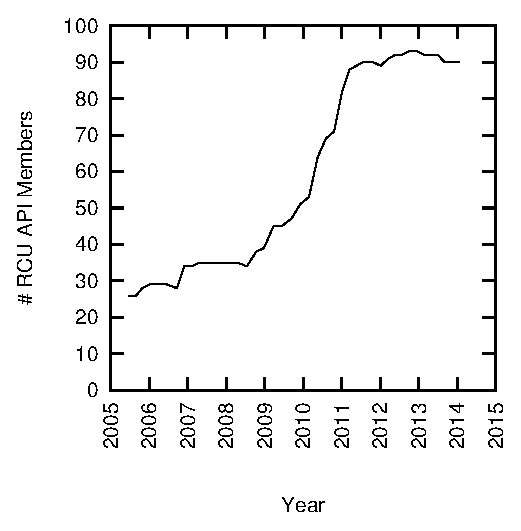
\includegraphics{appendix/rcuhist/rcuAPI}}
\end{center}
\caption{RCU API Growth Over Time}
\label{fig:app:rcuhist:RCU API Growth Over Time}
\end{figure}

Seven years of exposure to Linux increased the size of the RCU API from
the initial six components (seven if one counts explicit memory barriers)
to 31 components as of the Linux 2.6.24 kernel, as shown in
Figure~\ref{fig:app:rcuhist:RCU API Growth Over Time}.
Any way you calculate it, this is an extremely large increase in size,
an increase that was completely unexpected, given that the initial
DYNIX/ptx RCU API had been running in production supporting large datacenter
workloads for well over five years beforehand.
Of course, the Linux kernel has a variety of internal software environments,
including process context, interrupt context, and so on, which results
in more than 50 API members for simple locking.
However, DYNIX/ptx had a similar variety of internal software environments.

This situation therefore motivated a search for the reasons why a
technology so well-suited for datacenter workloads should require
so much change upon being introduced into Linux.
The lessons learned during this search are discussed in the next section.

\section{Lessons Learned}
\label{sec:app:rcuhist:Lessons Learned}

The experience of adapting RCU for Linux taught a number of valuable
lessons.
The first set of lessons pertained to working with
free/open source software (FOSS) communities, and
are covered in Section~\ref{sec:app:rcuhist:The Workings of FOSS Communities}.
Subsequent lessons are more specific to the evolution of the
RCU API, including
the wide range of workloads and platforms that Linux supports,
the use of Linux in networking infrastructure,
the economics of Linux's large community,
and the high degree of innovation fostered by the Linux community.
These RCU-specific lessons are covered by
Sections~\ref{sec:app:rcuhist:Wide Range of Workloads and Platforms} through
\ref{sec:app:rcuhist:Linux-Community Innovation}.

\subsection{The Workings of FOSS Communities}
\label{sec:app:rcuhist:The Workings of FOSS Communities}

Although my five-to-ten years with the Linux community by no means qualifies me
as an expert on the FOSS communities,
my combined experience with academia, research organizations,
proprietary software development groups, standards organizations,
and the Linux community does provide an interesting vantage point.
This section leverages this vantage point to describe how one might work
with the Linux community, drawing analogies with
situations that might be more familiar to many readers.

For example, consider a researcher working with a motivated
proprietary software vendor.
Such a vendor might make a particular developer responsible for
implementing the results of the research in the product.
This sort of relationship can also happen in FOSS projects,
for example, when Alexey Kuznetsov implemented stochastic fairness
queuing~\cite{McKenney90} in Linux---my only involvement in this
process was to send Alexey a copy of my paper.
Although this process can work extremely well, it depends on a developer
being ready, willing, and able to do the necessary work.
Such a developer might or might not be available.

FOSS projects permit another approach, namely, the researcher
downloading the project, making the necessary modifications, conducting
experiments, and reporting the results.
On the one hand, this approach eliminates the dependency on the developer,
but on the other hand it does nothing to foster inclusion of the researcher's
modifications into the FOSS project's official repository.
Such inclusion does require more work, but can greatly ease collaboration
and do much to advance the overall research agenda~\cite{MuliBenYehuda2008OSR}.

Although different projects have different criteria for inclusion,
even within the confines of the Linux community, it is well worthwhile
to consider the following questions:

\begin{enumerate}
\item	Does the value of your contribution exceed the cost of
	its inclusion in the FOSS project and its maintenance
	thereafter?
\item	Are there community members who are enthusiastic about
	your contribution?
\item	If community members invest the time and effort required
	to include your contribution, are you willing to make
	a compensating investment of your time and effort into
	the project?
\end{enumerate}

These questions are considered in the following sections.

\subsubsection{Code as Liability}
\label{sec:app:rcuhist:Code as Liability}

Source code is commonly considered to be an asset rather than a
liability.
After all, it can take great effort to produce, and can sometimes
be sold for considerable amounts of money.
The fallacy of the ``source code as asset'' viewpoint can be seen
by considering the fate of those unfortunates who purchase a body
of source code, but fail to retain the services of that code's developers.
Without the developers, it is often impossible to properly service,
support, and maintain the source code, possibly resulting in
bankruptcy or legal action.

It is often better to instead view the source code as a \emph{liability}
that one might be willing to incur only if the corresponding functionality
and performance is sufficiently valuable to the rest of the community.
Only then can the community be expected to continually invest the time
and effort required to fix the inevitable bugs, adapt the code to the
inevitable changes in the enclosing software environment, support the
users, add features demanded by those users, and so on.

In short, by incorporating your source-code contribution, the
project will be making an ongoing investment of time in effort
in order to give you your 15 minutes of fame and glory.
What will you give the project in return?

\subsubsection{Community Enthusiasm}
\label{sec:app:rcuhist:Community Enthusiasm}

The community might be willing (perhaps even happy) to accept your
source-code contribution if enough community members are enthusiastic about
the corresponding functionality or performance.
These members might be either developers or users.
This of course leads to the question of how to generate the
necessary enthusiasm.

One approach is to identify the community's enthusiasm
ahead of time, and then selecting a project that provides something that
the community badly wants or needs.
This approach can have the further advantage of garnering community
help and support during your research and implementation, and greatly
easing the inclusion process.
You should nevertheless take care to learn the community's culture and
coding style, and be prepared to interact with the community to shape
your contribution into a form consistent with community expectations.
You might also need to provide training and documentation to the
community in order to ease their learning and support burden.
With the proper preparation, this approach can be quite gratifying
to both the researcher and the community.

Another approach is to ``sell'' your contribution to the community,
either before or after creating it.
Although I have seen situations where this has worked well, I must
defer to those who have the relevant sales/marketing skills.

\subsubsection{Compensating Investments}
\label{sec:app:rcuhist:Compensating Investments}

In order to get your contribution included into a FOSS project, you might
need to invest some of your own time and effort to compensate the
community for the time and effort that they will incur supporting
and maintaining your contribution.
This is no different than the situation with any given academic journal:
authors are often expected to contribute their time and effort
acting as reviewers, and may in addition
need to be active members of the research community that the journal
serves.

FOSS communities also value review: contributors may be expected to
review and comment on the contributions of others, thereby increasing
the quality and robustness of the FOSS project.
Such efforts also build trust: a history of on-point reviews,
debugging, bug fixes, and
contributions that are consistent with the aims and culture of the project
will tend to increase the stature of the
contributor within that community.

However, the typical FOSS review process differs from the typical
academic process in a number of ways:

\begin{enumerate}
\item	FOSS reviews are not anonymous.
\item	Contributors can (and usually do) respond to FOSS reviews.
\item	Multiple contributors with similar goals will often collaborate
	to produce a single contribution that meets all their goals.
	This can also happen in academic circles, but the open nature
	of the FOSS review process more directly encourages such
	alliances.
\item	FOSS reviews can often be more harsh in tone than those in
	academic circles, though the effects of this harshness are
	balanced by the ability to respond directly and immediately.
\end{enumerate}

A developer who contributes to the review process (including debugging
and bug-fix efforts) will
earn the community's trust, and thus meet less resistance to
future contributions.
This situation is not all that different from an academic community.
As is the case with academic communities,
trust in one community does not necessarily immediately translate
to trust in another.
In particular, trust within an academic community
does not necessarily automatically translate to trust within the
corresponding FOSS community, and vice versa.
There are of course exceptions, one prominent example being Van Jacobson's
high level of esteem within the Linux-kernel networking community.

Within FOSS communities, as within most organizations, trust is key.
And, also like most organizations, one's level of trust is determined
by one's words and (especially) actions over time.

\subsubsection{FOSS Communities Summary}
\label{sec:app:rcuhist:FOSS Communities Summary}

The advent of FOSS communities is critically important, as they have
the potential of offering a publicly available bridge between research
and practice by offering researchers a way to test their ideas in
real-world software systems.
The fact that the FOSS projects are publicly available also allows
other researchers to easily replicate results, in happy contrast to
proprietary software.
FOSS communities also offer the prospect of academic research being
applied to practice in a timely manner, increasing the impact of
this research.

The following sections describe lessons that are more
specific to the Linux kernel.

\subsection{Wide Range of Workloads and Platforms}
\label{sec:app:rcuhist:Wide Range of Workloads and Platforms}

A key lesson learned from the RCU experience is that Linux runs
an incredible variety of workloads on a wide variety of platforms,
including embedded systems, cell phones, desktops, network processors,
servers, and supercomputers.
Each of these platforms brings its own set of issues and requirements,
a number of which affected RCU's design and implementation.
In particular, Linux runs real-time workloads, which required significant
changes to RCU, as described in
Sections~\ref{sec:app:rcuhist:Real-Time Systems, Part I} and
\ref{sec:app:rcuhist:Real-Time Systems, Part II}.
Furthermore, Linux is used in embedded systems with small memory,
which also affected RCU as described in Section~\ref{sec:app:rcuhist:Small-Memory Systems}.
Therefore, any technology that has been developed in a protected niche
is likely to require substantial changes in order to operate safely
and effectively in the less-protected Linux environment.

One advantage of the Linux kernel's FOSS nature is that not only
is the source code freely available, but that design discussions are also
freely available.
In fact, design discussions are open to general participation, the only
hard requirement being an ability to read and write English, 
but not necessarily to converse in spoken English.
To their credit, many researchers are already taking advantage of
this openness, using the Linux kernel as a platform for their research.
It is hoped that such collaborations will help to narrow the
researcher/practitioner divide, increasing the impact of research,
while speeding the evolution of the Linux kernel.

\subsection{Networking Infrastructure}
\label{sec:app:rcuhist:Networking Infrastructure}

In addition, Linux is heavily used in network infrastructure.
As noted earlier, this means that Linux cannot be protected
by a firewall because Linux \emph{is} the firewall.
Therefore, Linux must efficiently process networking loads that
might bring a machine designed for a carefully cossetted
datacenter environment to its knees.
This requirement had significant effects on the RCU API, as
noted in Sections~\ref{sec:app:rcuhist:Heavy Networking Loads} and
\ref{sec:app:rcuhist:Network-Based Denial-of-Service Attacks}.

\subsection{Software Development Economics}
\label{sec:app:rcuhist:Software Development Economics}

Economics also plays a part.
For example, there were only a few tens of kernel developers working
on DYNIX/ptx, perhaps 50 at most.
This means that an innovation in DYNIX/ptx that saved 1\% of each
developer's time would save at most six person-months per year.
If the innovation itself required one person-year to implement,
two years would be required to recover the cost of implementation.
Because there would be very likely be higher-payoff investments
of kernel-developer time, such an innovation might never be
implemented.

In contrast, many thousands of people work with the Linux kernel.
Even if we restrict our attention to people whose changes were
accepted into the 2.6.24 release of the Linux kernel, we end up
with 950~\cite{Corbet2008stats2:6:24}.
This smaller number does not count the number of people who read
kernel code to provide support, to fix bugs in older versions of
Linux, or to understand how best to implement Linux-based applications.
However, if we nevertheless take 1,000 as an estimate of the
number of full-time equivalent effort spent on the Linux kernel,
our one-person-year innovation could save ten person-years per
year, recovering the investment in not much more than a month.

This economic effect had a large effect on the
RCU API, for example, in the form of the RCU-based list-manipulation
primitives discussed in
Section~\ref{sec:app:rcuhist:Memory Barriers Unloved, Part I}.
Such primitives would likely have remained open-coded in operating
systems with smaller communities.
Because such primitives arguably increase productivity, it is
interesting to speculate on the long-term prospects of Linux
compared to kernels with communities having fewer active members.
Similar effects on the RCU API are described in
Sections~\ref{sec:app:rcuhist:Simplicity} and \ref{sec:app:rcuhist:Memory Barriers Unloved, Part II}.

\subsection{Linux-Community Innovation}
\label{sec:app:rcuhist:Linux-Community Innovation}

Arguably the largest effect was due to the highly innovative group of
developers in the Linux community, who applied RCU in a number of
ways, some completely unanticipated.
This is not necessarily to say that Linux developers are more innovative
than those in other environments (though the Linux community by no means
lacks extremely innovative and talented developers), but rather that
the widespread sharing of viewpoints in the open design process does
much to foster innovation.
Some of the effects of this innovation on RCU are covered in
\ref{sec:app:rcuhist:Unloadable Kernel Modules Use RCU},
\ref{sec:app:rcuhist:RCU Readers Must Block}, and
\ref{sec:app:rcuhist:RCU Readers of Lists Being Reaped}.
In addition, the drive towards simplicity discussed in
Section~\ref{sec:app:rcuhist:Simplicity} forced incremental adoption of RCU,
as described in
Section~\ref{sec:app:rcuhist:Linux Accepts RCU's Namesake}.

One can argue that Linux-community innovation will continue to drive
change into RCU, and into much else besides.
Such future prospects for RCU are taken up in the next section.

\section{Future Prospects}
\label{sec:app:rcuhist:Future Prospects}

Has every conceivable change to RCU already been made,
or will RCU continue to evolve?
This second view seems most likely.
And, although it is said that the best way to predict the future is to
invent it, it is also true that thinking a bit about the future can
help identify useful directions for invention.
The following sections therefore consider RCU-related issues in the areas
of power consumption, massively multicore systems,
real-time response, new synchronization primitives,
and, finally,
RCU API orthogonality.

\subsection{Power Consumption}
\label{sec:app:rcuhist:Power Consumption}

There has been some progress over the past year better integrating
preemptible RCU (the real-time variant) with the dynamic ticks
power-conservation feature (selected by the
\co{CONFIG_NO_HZ} Linux kernel parameter).
The idea behind dynamic ticks is that idle CPUs should forgo the
scheduling-clock interrupt, allowing them to reach deeper ``sleep
states'', thus better conserving power.

Unfortunately, older versions of preemptible RCU would awaken all
CPUs, including those in sleep states, whenever an RCU updater 
required an RCU grace period to elapse.
This problem was addressed by a new interface
between dynamic ticks and RCU that avoids waking
sleeping CPUs~\cite{SteveRostedt2008dyntickRCUpatch}.
This same technique could profitably be applied to other
implementations of RCU as well.

\subsection{Massively Multicore Systems}
\label{sec:app:rcuhist:Massively Multicore Systems}

Increased CPU counts might require that the scalability
of RCU's grace-period detection be improved (and much else besides).
Although the original ``classic'' implementation of RCU has
been modified to run efficiently on a 512-CPU Altix machine~\cite{Spraul04a},
other variants would require more work to run well on systems with
large numbers of CPUs.
Spraul's hierarchical approach has proven successful in other
environments, and is likely to be the method
of choice on very large systems.

However, if per-chip CPU counts were to rise without limit,
then it is entirely possible that memory bandwidth and on-chip cache size
will fail to increase sufficiently to permit some workloads from
taking full advantage of all of the CPUs.
A rational response to this situation might well be to simply
avoid using some fraction of these (presumably extremely low-cost) CPUs.
However, power-consumption issues might motivate
high CPU utilization in order to minimize the total number of systems
required for a given workload.
If such a situation arises,
memory conservation might well be required on large machines
as well as on tiny embedded systems.

Such a need for memory conservation would further increase the motivation
to shrink the \co{rcu_head}
structure by tabulating RCU callback functions and encoding the
resulting table index into this structure's pointer to
next~\cite{PaulEMcKenney2006b}, thereby reducing the memory footprint
of heavily replicated RCU-protected data structures, such as
those making up the directory-entry cache.

Of course, increased focus on memory footprint would undoubtably affect
many other aspects of the Linux kernel as well.

\subsection{Real-Time Response}
\label{sec:app:rcuhist:Real-Time Response}

The need for improved real-time response has already had a large
effect on RCU, as discussed in
Sections~\ref{sec:app:rcuhist:Real-Time Systems, Part I} and
\ref{sec:app:rcuhist:Real-Time Systems, Part II}.
It seems likely that increasingly aggressive real-time response constraints
will be applied to additional areas within the Linux kernel.
For example, the advent of low-cost, high-capacity, and low-latency
solid-state storage removes the traditional seek-time and rotational-latency
barriers to real-time mass-storage access.
This turn of events may well raise interest in real-time mass storage
access, both with and without filesystems.
RCU might well have a role to play in this arena, which in turn might
require changes to RCU, either in the RCU infrastructure itself
or in the way that RCU is used and applied.

Increasing bandwidths and decreasing latencies of data-communications
hardware seem quite likely to have the same effect on Linux's
protocol stacks.

In addition, as multi-core CPUs continue to gain popularity in real-time
systems, we may possibly see a need for RCU in user applications, at
least for those applications written in non-garbage-collected languages
such as C and C++.

However, it is important to note that real-time RCU work to date has
focused almost entirely on RCU's read-side primitives.
When performing RCU updates, it is often necessary to defer destructive
actions (such as freeing memory previously removed from an RCU-protected
data structure) until all pre-existing RCU readers have completed.
The length of time that such actions must be deferred is known as an
``RCU grace period''.
In some RCU implementations, these grace periods can extend for tens of
milliseconds~\cite{DinakarGuniguntala2008IBMSysJ}, which can sometimes
be inconveniently
long~\cite{JensAxboe2006SlowSRCU,PeterZijlstra2007SyncBarrier}.

This situation inspired a new implementation of RCU that favors updates,
named QRCU~\cite{PaulMcKenney2007QRCUpatch,
PaulEMcKenney2007QRCUspin,OlegNesterov2006QRCU}.
However, QRCU has not yet been accepted into the Linux kernel, and
might or might not ever be.
There has also been discussion of mechanisms to expedite grace-period
computation for existing RCU implementations, perhaps providing RCU API
members such as \co{synchronize_rcu_expedited()}.
Many open questions remain in this area.

\subsection{New Synchronization Primitives}
\label{sec:app:rcuhist:New Synchronization Primitives}

RCU is a specialized synchronization primitive that is intended for
use in read-mostly situations or in situations requiring deterministic
readers.
Because RCU is not so foolish as to attempt to be all things to all
developers in all situations, it must interface conveniently and
efficiently with other synchronization mechanisms.
RCU has a long history of interfacing well with lock-based updates, and has
also seen extensive use interfacing with atomic-instruction-based updates.
There have also been some successful experiments interfacing RCU
with non-blocking-synchronization-based
updates~\cite{PaulEdwardMcKenneyPhD}.

More recently, researchers have attempted to interface RCU to
transactional-memory-based update, however, early attempts
resulted in RCU readers unnecessarily aborting transactional
updates~\cite{ChistopherJRossbach2007a}.
More recent work avoids this problem, but restricts the transactional-memory
implementation.
Should transactional memory graduate from research to practice, more
work will be needed to interface it efficiently with RCU.

\subsection{RCU API Orthogonality}
\label{sec:app:rcuhist:RCU API Orthogonality}

\begin{table*}[tb]
\begin{center}
\scriptsize
\begin{tabular}{l||l|l|l}
Category  & Publish	& Retract	& Subscribe \\
\hline
\hline
Pointers  & \co{rcu_assign_pointer()}
			& \co{rcu_assign_pointer(..., NULL)}
					& \co{rcu_dereference()} \\
\hline
Lists     & \parbox{1.5in}{
		\co{list_add_rcu()} $\strut$  \\
		\co{list_add_tail_rcu()} \\
		\co{list_replace_rcu()} $\strut$ }
			& \co{list_del_rcu()}
					& \co{list_for_each_entry_rcu()} \\
\hline
Hlists    & \parbox{1.5in}{
		\co{hlist_add_after_rcu()} $\strut$ \\
		\co{hlist_add_before_rcu()}  \\
		\co{hlist_add_head_rcu()} \\
		\co{hlist_replace_rcu()} $\strut$ }
			& \co{hlist_del_rcu()}
					& \co{hlist_for_each_entry_rcu()}
\end{tabular}
\end{center}
\caption{RCU Publish and Subscribe Primitives}
\label{tab:app:rcuhist:RCU Publish and Subscribe Primitives}
\end{table*}

\begin{table*}[tb]
\begin{center}
\scriptsize
\begin{tabular}{l||l|l|l|l}
 & RCU Classic & RCU BH & RCU Sched & SRCU \\
\hline
\hline
Read-Side Primitives
	& \parbox{1.0in}{
		\co{rcu_read_lock()} \\
		\co{rcu_read_unlock()}}
		& \parbox{1.0in}{
			\co{rcu_read_lock_bh()} \\
			\co{rcu_read_unlock_bh()}}
			& \parbox{1.0in}{
				\co{preempt_disable()} $\strut$ \\
				\co{preempt_enable()} \\
				and friends $\strut$}
				& \parbox{1.0in}{
					\co{srcu_read_lock()} \\
					\co{srcu_read_unlock()}} \\
\hline
\parbox{1.3in}{\raggedright Update-Side~Primitives $\strut$ (Synchronous) $\strut$}
	& \parbox{1.0in}{
		\co{synchronize_rcu()} $\strut$ \\
		\co{synchronize_net()} $\strut$ }
			&
				& \co{synchronize_sched()}
					& \co{synchronize_srcu()} \\
\hline
\parbox{1.3in}{\raggedright Update-Side~Primitives $\strut$ (Asynchronous) $\strut$}
	& \co{call_rcu()}
		& \co{call_rcu_bh()}
			& 
				& N/A \\
\hline
Update-Side Barriers
	& \co{rcu_barrier()}
		& 
			& 
				& N/A \\
\end{tabular}
\end{center}
\caption{RCU Read- and Update-Side Primitives}
\label{tab:app:rcuhist:RCU Read- and Update-Side Primitives}
\end{table*}

The RCU API is currently not orthogonal:
a tabulation of the RCU API shown in
Tables~\ref{tab:app:rcuhist:RCU Publish and Subscribe Primitives} and
\ref{tab:app:rcuhist:RCU Read- and Update-Side Primitives}
reveals several missing members, namely \co{synchronize_rcu_bh()}
(the synchronous counterpart to \co{call_rcu_bh()}),
\co{call_rcu_sched()} (the asynchronous counterpart to
\co{synchronize_sched()}),
\co{rcu_barrier_sched()} (the barrier counterpart to \co{call_rcu_bh()}),
and
\co{rcu_barrier_bh()} (the barrier counterpart to \co{call_rcu_sched()}).

Of course, orthogonality alone is not necessarily sufficient to motivate
adding code to the Linux kernel.
However, a need for \co{call_rcu_sched()} and \co{rcu_barrier_sched()}
has recently arisen~\cite{MathieuDesnoyers2007call:rcu:schedNeeded},
which might result in adding this pair of interfaces.

It is of course unwise to measure the capability of a technology such
as RCU by the number of elements in its API.
In fact, a reduction in the size of the RCU API would undoubtably be
quite welcome.
There is at least a theoretical possibility of substantial
convergence~\cite{ChristophHellwig2006RCU2SRCU},
but the question remains open as to whether SRCU can subsume all
the functionality of the other forms of RCU,
while still providing adequate performance.

\section{Conclusions}
\label{sec:app:rcuhist:Conclusions}

Introducing RCU into Linux forced dramatic and unexpected change into RCU,
for example, expanding the RCU API from six members in 2001
to more than 30 members in 2007.
There is reason to believe that Linux will continue forcing change
into RCU, in particular, one welcome change would be a slower increase, or
better yet a decrease, in the size of the RCU API.

These additions occurred a few at a time, and were motivated by
the increasingly wide range of workloads and platforms that
Linux supports,
the use of RCU in networking infrastructure,
the economics of Linux's large community,
and the high degree of innovation fostered by the Linux community.
To give only one example,
although datacenters tend to be protected by firewalls,
Linux cannot assume firewall protection because Linux \emph{is} the firewall.
Therefore, technologies developed in protected datacenter environments
will likely require significant overhauls when being adapted to Linux,
and it in fact seems likely that Linux will require continued changes
to RCU.
It seems likely that RCU's experience applies to other technologies
that might be introduced to the Linux kernel.

Nevertheless, the opportunity to work on an artifact as widely used as
is Linux is a rare privilege, and working on Linux's RCU implementation
continues to be a deeply rewarding learning experience.

And, as the following section demonstrates,
it is also an ongoing learning experience.

\section{Epilog}
\label{sec:app:rcuhist:Epilog}

This section presents ongoing experience with RCU subsequent to initial
publication of this paper in mid-2008~\cite{PaulEMcKenney2008RCUOSR}.

\subsection{2.6.27 Linux Kernel}

This release added the
\co{call_rcu_sched()},
\co{rcu_barrier_sched()}, and
\co{rcu_barrier_bh()} RCU API members,
and predicted in Section~\ref{sec:app:rcuhist:RCU API Orthogonality}.

\subsection{2.6.28 Linux Kernel}

One welcome change involved an actual reduction in the size of RCU's
API with the removal of the \co{list_for_each_rcu()} primitive.
This primitive is superseded by \co{list_for_each_entry_rcu()},
which has the advantage of iterating over structures rather than
iterating over the pointer pairs making up a \co{list_head}
structure (which, confusingly, acts as a list element as well
as a list header).
This change was accepted into the 2.6.28 Linux kernel.

Unfortunately, the 2.6.28 Linux kernel also added some RCU API
members, namely, \co{rcu_read_lock_sched()} and
\co{rcu_read_unlock_sched()}, which Section~\ref{sec:app:rcuhist:RCU API Orthogonality}
somehow failed to anticipate.
These APIs were added to promote readability.
In the past, primitives to disable interrupts or preemption were used
to mark the RCU read-side critical sections corresponding to
\co{synchronize_sched()}.
However, this practice led to bugs when developers removed the need
to disable preemption or interrupts, but failed to notice the need
for RCU protection.
Use of \co{rcu_read_lock_sched()} will help prevent such bugs in the
future.

\subsection{2.6.29 Linux Kernel}

A new more-scalable implementation, dubbed ``Tree RCU'', replaces
the flat bitmap with a combining tree, and was accepted into the 2.6.29
Linux kernel.
This implementation was inspired by the ever-growing core counts of
modern multiprocessors (see Section~\ref{sec:app:rcuhist:Massively Multicore Systems},
and is designed for many hundreds of CPUs.
Its current architectural limit is 262,144 CPUs, which the authors
(perhaps na\"ively) believe to be sufficient for quite some time.
This implementation also adopts preemptible RCU's improved dynamic-tick
interface (see Section~\ref{sec:app:rcuhist:Power Consumption}).

Mathieu Desnoyers added
\co{rcu_read_lock_sched_notrace()} and
\co{rcu_read_unlock_sched_notrace()},
which are required to permit the tracing code in the Linux kernel
to use RCU.
Without these APIs, attempts to trace RCU read-side critical sections
lead to infinite recursion.

Eric Dumazet added a new type of RCU-protected list that allows single-bit
markers to be stored in the list pointers.
This type of list enables a number of lockless algorithms, including
some reported on by Maged Michael~\cite{MagedMichael04a}.
Eric's work adds the \co{hlist_nulls_add_head_rcu()},
\co{hlist_nulls_del_rcu()}, \co{hlist_nulls_del_init_rcu()}, and
\co{hlist_nulls_for_each_entry_rcu()}.
It also adds a new structure named \co{hlist_nulls_node}.

Although it is strictly speaking not part of the Linux kernel, 
at about this same time, Mathieu Desnoyers announced his user-space
RCU implementation~\cite{MathieuDesnoyers2009URCU}.
This is an important first step towards the real-time user-level RCU
implementation discussed in
Section~\ref{sec:app:rcuhist:Real-Time Response}.

\subsection{2.6.31 Linux Kernel}

Jiri Pirko added \co{list_entry_rcu} and \co{list_first_entry_rcu()}
primitives that encapsulate the \co{rcu_dereference()} RCU-subscription
primitive into higher-level list-access primitives, which will hopefully
eliminate a class of bugs.

In addition, the ``Tree RCU'' implementation was upgraded from
``experimental'' status.

\subsection{2.6.32 Linux Kernel}

Perhaps the largest change in this version of the Linux kernel
is the removal of the old ``Classic RCU'' implementation.
This implementation is superseded by the ``Tree RCU'' implementation.

This version saw a number of other changes, including:

\begin{enumerate}
\item	The \co{synchronize_rcu_expedited()} RCU API member discussed
	in Section~\ref{sec:app:rcuhist:Real-Time Response}, along with
	\co{synchronize_sched_expedited()} as well as
	\co{synchronize_rcu_bh_expedited()}.
	These primitives are equivalent to their non-expedited
	counterparts, except that they take measures to expedite the
	grace period.
\item	Add preemptible-RCU functionality to the ``Tree RCU''
	implementation, thus removing one obstacle to real-time
	response from large multiprocessor machines running Linux.
\item	This new ``Tree Preemptible RCU'' implementation obsoletes
	the old preemptible RCU implementation, which was removed
	from the Linux kernel.
\end{enumerate}

\subsection{2.6.33 Linux Kernel}

Perhaps the most dramatic addition to this release was
a day-one bug in Tree RCU~\cite{PaulEMcKenney2009HuntingHeisenbugs}.
Other changes include:

\begin{enumerate}
\item	``Tiny RCU'', also known as ``RCU: The Bloatwatch
	Edition''~\cite{PaulEMcKenney2009LWNBloatWatchRCU}.
\item	Expedited SRCU in the form of
	\co{synchronize_srcu_expedited()}.
\item	A cleanup of Tree RCU synchronization prompted by the
	afore-mentioned bug.
\item	Add expedited implementation for Tree Preemptible RCU
	(in earlier releases, ``expedited'' support had simply
	mapped to \co{synchronize_rcu()}, which is semantically
	correct if somewhat unhelpful from a performance viewpoint.)
\item	Add a fourth level to Tree RCU, which improves stress testing.
	Therefore, if someone ever wants to run Linux on a system with
	16,777,216 CPUs, RCU is ready for them!
	Give or take the response-time implications of scanning
	through 16 million per-CPU data elements...
\end{enumerate}

\subsection{2.6.34 Linux Kernel}

The most visible addition for this release was \co{CONFIG_PROVE_RCU},
which allows \co{rcu_dereference()} to check for correct locking
conditions~\cite{PaulEMcKenney2010LockdepRCU}.
Other changes include:

\begin{enumerate}
\item	Simplifying Tree RCU's interactions between
	forcing an old grace period and starting a new one.
\item	Rework counters so that free-running counters are unsigned.
	(You simply cannot imagine the glee on the faces of certain
	C-compiler hackers while they discussed optimizations that would
	break code that naively overflowed signed integers!!!)
\item	Update Tree Preemptible RCU's stall detection to print out
	any tasks preempted for excessive time periods while in
	an RCU read-side critical section.
\item	Other bug fixes and improvements to Tree RCU's CPU-stall-detection
	code.
	This code checks for CPUs being locked up, for example,
	in infinite loops with interrupts disabled.
\item	Prototype some code to accelerate grace periods when the
	last CPU goes idle in battery-powered multiprocessor
	systems.
	There were people who were quite unhappy about RCU taking
	a few extra milliseconds to get the system in a state
	where all CPUs could be powered down!
\end{enumerate}

\subsection{2.6.35 Linux Kernel}

This release includes a number of bug fixes and cleanups.
The major change is the first installment of Mathieu Desnoyers's
patch to check for misuse of RCU callbacks, for example, passing
a \co{rcu_head} structure to \co{call_rcu()} a second time within
a single grace period.

\subsection{2.6.36 Linux Kernel}

The core of Mathieu Desnoyers's debugobjects work appeared in 2.6.36,
with some cleanups deferred to 2.6.37 due to dependencies on commits
flowing up other maintainer trees.
A key piece of Arnd Bergmann's sparse RCU checking appeared in 2.6.36,
with the remainder deferred to 2.6.37, again due to dependencies on
commits flowing up other maintainer trees.
Finally, a patch from Eric Dumazet fixed an error in
\co{rcu_dereference_bh()}'s error checking.

\subsection{2.6.37 Linux Kernel}

The final cleanups from Mathieu Desnoyers's debugobjects work appeared
in 2.6.37, as did the remainder of Arnd Bergmann's sparse-based checking work.
Lai Jiangshan added some preemption nastiness to rcutorture and
made some simplifications to Tree RCU's handling of per-CPU data.
Tetsuo Handa fixed an RCU lockdep splat, Christian Dietrich removed
a redundant \co{#ifdef}, and Dongdong Deng added an
\co{ACCESS_ONCE()} that help call out lockless accesses to some
Tree RCU control data.

Paul's implementation of preemptible Tiny RCU also appeared in
2.6.37, as did a number of enhancements to the RCU CPU stall-warning
code, docbook fixes, coalescing of duplicate code, Tree RCU speedups,
added tracing to support queuing models on RCU callback flow,
and several miscellaneous fixes and cleanups.

\subsection{2.6.38 Linux Kernel}

Lai Jiangshan moved \co{synchronize_sched_expedited()} out of
\co{kernel/sched.c} and into \co{kernel/rcutree.c} and
\co{kernel/rcu_tiny.c} where it belongs.
He also simplified RCU-callback handling during CPU-hotplug operations
by eliminating the \co{orphan_cbs_list}, so that RCU callbacks
orphaned by a CPU that is going offline are immediately adopted by
the CPU that is orchestrating the offlining sequence.
Tejun Heo improved \co{synchronize_sched_expedited()}'s batching
capabilities, which in turn improves performance and scalability
for workloads with many concurrent \co{synchronize_sched_expedited}
operations.
Frederic Weisbecker provided a couple of subtle changes to the
RCU core code that make RCU more power-efficient when idle.
Mariusz Kozlowski fixed an embarrassing syntax error in
\co{__list_for_each_rcu()}, which was then removed.
(But the fixed version is there in the git tree should it be needed.)
Nick Piggin added the \co{hlist_bl_set_first_rcu()},
\co{hlist_bl_first_rcu()},
\co{hlist_bl_del_init_rcu()},
\co{hlist_bl_del_rcu()},
\co{hlist_bl_add_head_rcu()}, and
\co{hlist_bl_for_each_entry_rcu()} primitives for RCU-protected use
of bit-locked doubly-linked lists.
Christoph Lameter implemented \co{__this_cpu_read()}, which is an
optimized variant of
\co{__get_cpu_var()} for use in cases where the variable is accessed directly.

In addition, \co{TINY_RCU} gained priority boosting, a race condition
in \co{synchronize_sched_expedited()} was fixed,
\co{synchronize_srcu_expedited()} was modified to retain its expedited
nature in the face of concurrent readers,
grace-period begin/end checks were improved,
and the \co{TREE_RCU} leaf-level fanout was limited to 16 in order to fix
lock-contention problems.

\subsection{2.6.39 Linux Kernel}

Lai Jiangshan made \co{TINY_RCU}'s \co{exit_rcu()} invoke
\co{__rcu_read_unlock()}
rather than \co{rcu_read_unlock()} in case of a task exiting while
in an RCU read-side critical section in order to preserve debugging
state,
Jesper Juhl removed a duplicate include of \co{sched.h} from
rcutorture,
and
Amerigo Wang removed some dead code from \co{rcu_fixup_free()}.

In addition, a new \co{rcu_access_index()} was created for use in the
MCE subsystem.

\subsection{What Comes After 2.6.39?}

At long last, priority boosting for Tree RCU should appear in 2.6.40.

Mathieu Desnoyers enabled \co{DEBUG_OBJECTS_RCU_HEAD} checking to
be carried out in non-preemptible RCU implementations.
Lai Jiangshan created a fire-and-forget \co{kfree_rcu()} (and applied
it throughout the kernel),
and also made \co{TREE_RCU}'s \co{exit_rcu()} invoke
\co{__rcu_read_unlock()}
rather than \co{rcu_read_unlock()} in case of a task exiting while
in an RCU read-side critical section in order to preserve debugging
state.
Eric Dumazet further shrunk \co{TINY_RCU} and applied the new
\co{kthread_create_on_node()} primitive to ensure that RCU's
kthreads have memory placed optimally on NUMA systems.
Gleb Natapov added RCU hooks to allow virtualization to call RCU's
attention to quiescent states that occur when switching context to
and from a guest OS.
Peter Zijlstra streamlined RCU kthread blocking and wakeup.

The design for pulling SRCU into the Tree RCU implementation is still
looking reasonably good, aside from interactions with the soft-lockup code.
However, it will still likely be a few releases before SRCU is pulled
into Tree RCU and Tiny RCU.

There has been an initial request for \co{rcu_barrier_expedited()},
but given that the requester found another way to solve this problem,
this has relatively low priority.
